\chapter{\IfLanguageName{dutch}{Stand van zaken}{State of the art}}%
\label{ch:stand-van-zaken}

% Tip: Begin elk hoofdstuk met een paragraaf inleiding die beschrijft hoe
% dit hoofdstuk past binnen het geheel van de bachelorproef. Geef in het
% bijzonder aan wat de link is met het vorige en volgende hoofdstuk.

% Pas na deze inleidende paragraaf komt de eerste sectiehoofding.

% Dit hoofdstuk bevat je literatuurstudie. De inhoud gaat verder op de inleiding, maar zal het onderwerp van de bachelorproef *diepgaand* uitspitten. De bedoeling is dat de lezer na lezing van dit hoofdstuk helemaal op de hoogte is van de huidige stand van zaken (state-of-the-art) in het onderzoeksdomein. Iemand die niet vertrouwd is met het onderwerp, weet nu voldoende om de rest van het verhaal te kunnen volgen, zonder dat die er nog andere informatie moet over opzoeken \autocite{Pollefliet2011}.

% Je verwijst bij elke bewering die je doet, vakterm die je introduceert, enz.\ naar je bronnen. In \LaTeX{} kan dat met het commando \texttt{$\backslash${textcite\{\}}} of \texttt{$\backslash${autocite\{\}}}. Als argument van het commando geef je de ``sleutel'' van een ``record'' in een bibliografische databank in het Bib\LaTeX{}-formaat (een tekstbestand). Als je expliciet naar de auteur verwijst in de zin (narratieve referentie), gebruik je \texttt{$\backslash${}textcite\{\}}. Soms is de auteursnaam niet expliciet een onderdeel van de zin, dan gebruik je \texttt{$\backslash${}autocite\{\}} (referentie tussen haakjes). Dit gebruik je bv.~bij een citaat, of om in het bijschrift van een overgenomen afbeelding, broncode, tabel, enz. te verwijzen naar de bron. In de volgende paragraaf een voorbeeld van elk.

% \textcite{Knuth1998} schreef een van de standaardwerken over sorteer- en zoekalgoritmen. Experten zijn het erover eens dat cloud computing een interessante opportuniteit vormen, zowel voor gebruikers als voor dienstverleners op vlak van informatietechnologie~\autocite{Creeger2009}.

% Let er ook op: het \texttt{cite}-commando voor de punt, dus binnen de zin. Je verwijst meteen naar een bron in de eerste zin die erop gebaseerd is, dus niet pas op het einde van een paragraaf.

% \begin{figure}
%   \centering
%   
\includegraphics[width=0.8\textwidth]{grail.jpg}
%   \caption[Voorbeeld figuur.]{\label{fig:grail}Voorbeeld van invoegen van een figuur. Zorg altijd voor een uitgebreid bijschrift dat de figuur volledig beschrijft zonder in de tekst te moeten gaan zoeken. Vergeet ook je bronvermelding niet!}
% \end{figure}

% \begin{listing}
%   \begin{minted}{python}
%     import pandas as pd
%     import seaborn as sns

%     penguins = sns.load_dataset('penguins')
%     sns.relplot(data=penguins, x="flipper_length_mm", y="bill_length_mm", hue="species")
%   \end{minted}
%   \caption[Voorbeeld codefragment]{Voorbeeld van het invoegen van een codefragment.}
% \end{listing}

% \lipsum[7-20]

% \begin{table}
%   \centering
%   \begin{tabular}{lcr}
%     \toprule
%     \textbf{Kolom 1} & \textbf{Kolom 2} & \textbf{Kolom 3} \\
%     $\alpha$         & $\beta$          & $\gamma$         \\
%     \midrule
%     A                & 10.230           & a                \\
%     B                & 45.678           & b                \\
%     C                & 99.987           & c                \\
%     \bottomrule
%   \end{tabular}
%   \caption[Voorbeeld tabel]{\label{tab:example}Voorbeeld van een tabel.}
% \end{table}

Als modern IT bedrijf is het belangrijk om de veiligheid van data te garanderen als ook snelle, en betrouwbare toegang tot applicaties en diensten te bieden. Dit is de reden waarom het bedrijf heeft gekozen voor een SASE architectuur.

\vspace{2ex}

Deze studie onderzoekt de implementatie van een SASE-architectuur binnen de hybride cloudomgeving van een softwarebedrijf gebruikmakend van het Netskope platform. 

\vspace{2ex}

Als eerste stap in dit onderzoek is het belangrijk om de huidige situatie van het bedrijf te analyseren. Dit omvat een overzicht van de netwerk- en security-uitdagingen samen met de tekortkomingen in de huidige architectuur.

\section{Wat is SASE?}
Secure Access Service Edge (SASE) is een cloud-gebaseerd beveiligingsmodel dat netwerk- en beveiligingsfuncties combineert in één geïntegreerd platform. Deze technologie is ontstaan als antwoord op de toenemende complexiteit van moderne IT-infrastructuren, waarbij bedrijven steeds meer vertrouwen op cloud-diensten en gedistribueerde werkplekken.

\vspace{2ex}

SASE biedt een oplossing die traditionele netwerkmuren doorbreekt door beveiligde toegang te verlenen aan gebruikers, ongeacht hun locatie of het apparaat dat ze gebruiken~\autocite{KPN2023}.

\vspace{2ex}

SASE is een relatief nieuw framework dat netwerk- en beveiligingsfuncties samenvoegt in één cloudgebaseerd servicemodel. Het wordt steeds belangrijker, vooral in omgevingen waar gebruikers en data zich nu buiten het traditionele netwerkperimeter bevinden. 

\vspace{2ex}

SASE combineert SD-WAN (Software-Defined Wide Area Networking) technologie voor netwerkoptimalisatie met cloudgebaseerde beveiligingsfuncties, waaronder Zero Trust Network Access (ZTNA), Cloud Access Security Brokers (CASB) en Firewall-as-a-Service (FWaaS)~\autocite{ZPE2025}.

\section{Het gekozen platform, Netskope}
Netskope is gekozen als het platform voor de implementatie van een SASE-architectuur binnen de hybride cloudomgeving van het bedrijf. Netskope onderscheidt zich door zijn geïntegreerde benadering van netwerk- en beveiligingsdiensten via het Netskope One Platform. 

\vspace{2ex}

Dit platform combineert geavanceerde technologieën zoals de Zero Trust Engine, NewEdge-netwerk en uitgebreide DLP-functionaliteiten om zowel beveiliging als connectiviteit te optimaliseren~\autocite{Netskope2025-1}.

\subsection{Kernpijlers}
De SASE-architectuur van Netskope rust op vier essentiële kernpijlers die samen een omvattend beveiligingsraamwerk vormen, specifiek afgestemd op de uitdagingen van moderne hybride cloudomgevingen zoals die van een software agency bedrijf:

\begin{itemize}
  \item \textbf{Zero Trust Engine}: Deze kerncomponent biedt contextbewuste beveiliging door risico's in real-time te analyseren op basis van meer dan 50 variabelen, zoals gebruikersgedrag, apparaatprofielen en applicatiecontext. Dit stelt organisaties in staat om adaptieve toegangscontrole toe te passen en risico's proactief te beheren~\autocite{Netskope2025-2}.
  \item \textbf{NewEdge-netwerk}: Het grootste private cloudnetwerk ter wereld biedt lage latentie en optimale prestaties voor SaaS-applicaties, webverkeer en privétoepassingen. Dit netwerk maakt gebruik van uitgebreide peeringrelaties om snelle toegang te garanderen zonder prestatieverlies~\autocite{Netskope2025-1}.
  \item \textbf{DLP}: Netskope biedt uitgebreide databescherming door middel van AI-gestuurde detectie en classificatie van gevoelige gegevens over netwerken, endpoints en cloudomgevingen~\autocite{Netskope2025-1}.
  \item \textbf{Geïntegreerde SD-WAN}: Voor het optimaliseren van netwerken op locatie en het verbinden van filialen met de cloud via veilige verbindingen~\autocite{Netskope2025-1}.
\end{itemize}

\subsection{Waarom Netskope?}
In tegenstelling tot andere SASE-leveranciers biedt Netskope een volledig geïntegreerd platform zonder afhankelijkheid van meerdere leveranciers of gefragmenteerde oplossingen. Dit vermindert operationele complexiteit, verbetert de gebruikerservaring en zorgt voor consistente beleidsimplementatie over alle netwerk- en beveiligingslagen heen~\autocite{Netskope2025-1}.

\vspace{2ex}

Met deze geïntegreerde aanpak biedt Netskope een robuuste oplossing voor bedrijven die willen overstappen naar een modern SASE-model. Het platform combineert geavanceerde technologieën met schaalbare architectuur, wat essentieel is voor het waarborgen van veiligheid, prestaties en compliance in hybride omgevingen.

\section{Zero Trust}
Zero Trust is een model dat gebaseerd is op de stelling dat geen enkel apparaat, gebruiker of systeem automatisch te vertrouwen is, zelfs niet als deze zich binnen het netwerk bevinden~\autocite{Netskope2024}.

\vspace{2ex}

De nadruk ligt op het continu verifiëren van gebruikersidentiteit, het beperken van toegang tot strikt noodzakelijke bronnen (least privileged access), en het monitoren van netwerkactiviteiten om verdachte handelingen snel te identificeren en aan te pakken.

\vspace{2ex}

Volgens Microsoft is de kern van het Zero Trust-model gebaseerd op drie belangrijke principes: altijd verifiëren, nooit vertrouwen; minimaal toegang verlenen; en schade beperken bij inbreuk. Dit houdt in dat de toegang tot systemen of data niet alleen wordt beperkt op basis van de locatie van de gebruiker of het apparaat, maar altijd afhangt van de identiteit, rol en andere specifieke toegangsbeperkingen~\autocite{Microsoft2024}. 

\vspace{2ex}

Kaspersky benadrukt het belang van de technologieën die Zero Trust mogelijk maken, zoals multi-factor authenticatie (MFA), versleuteling van communicatie en geavanceerde netwerkmonitoringtool. ``De omslag naar hybride werken en de toename van het aantal cyberbedreigingen die ook nog eens steeds complexer worden, betekent dat cyberweerbaarheid voor veel organisaties de hoogste prioriteit heeft.'' Cyberweerbaarheid houdt in dat we onze focus moeten verleggen van preventie van cyberaanvallen naar de acceptatie dat dit soort aanvallen tegenwoordig onvermijdelijk zijn en we ervoor moeten zorgen dat organisaties zo goed mogelijk zijn voorbereid op eventuele aanvallen en snel en effectief kunnen herstellen. Zero Trust speelt een belangrijke rol in verbeterde cyberweerbaarheid~\autocite{Kaspersky2024}.

\vspace{2ex}

NIST definieert \textbf{Zero Trust Architecture (ZTA)} als een volledig cybersecurity-plan dat vertrouwen nooit impliciet verleent, maar continu evalueert. ZTA richt zich op het beschermen van alle resources – van gegevensbronnen tot netwerkapparatuur – door strikte authenticatie, autorisatie en encryptie toe te passen bij elke toegangsverzoek~\autocite{NIST2020}.

\subsection{Kernprincipes van Zero Trust}
\label{sec:Kernprincipes van Zero Trust}
Zeven fundamentele principes vormen de basis van NIST’s Zero Trust-architectuur~\autocite{NIST2020}:  

\begin{itemize}
  \item \textbf{Alle resources als entiteiten beschouwen}: Zowel kleine apparaten als complexe systemen worden behandeld als beveiligingsobjecten die specifieke controles vereisen.  
  \item \textbf{Beveiligde communicatie ongeacht locatie}: Netwerksegmentatie biedt geen automatisch vertrouwen; zelfs interne apparaten moeten aan dezelfde beveiligingseisen voldoen als externe.  
  \item \textbf{Toegang per sessie}: Vertrouwen in de aanvrager wordt geëvalueerd vóór toegang wordt verleend, met minimale rechten om een taak uit te voeren.  
  \item \textbf{Dynamisch beleid}: Toegang wordt gebaseerd op contextuele factoren zoals identiteit, apparaatstatus, gedragsanalyse en omgevingsvariabelen.  
  \item \textbf{Continue monitoring van integriteit}: Geen enkel apparaat wordt blind vertrouwd; beveiligingsstatus wordt bij elke aanvraag gecontroleerd.  
  \item \textbf{Dynamische authenticatie en autorisatie}: Validatie gebeurt tijdens de sessie, met mogelijkheid tot herauthenticatie bij ongewoon gedrag.  
  \item \textbf{Maximale informatieverzameling}: Zichtbaarheid over assets, netwerkverkeer en gebruikersactiviteiten dient als input voor risico-evaluatie en beleidsaanpassing.  
\end{itemize}

\subsection{Implementatiestrategieën}
NIST raadt drie benaderingen aan voor migratie naar ZTA~\autocite{NIST2020}:

\begin{itemize}
  \item \textbf{Versterkt identiteitsbeheer}: Identiteit als kerncomponent voor toegangsbeslissingen, gekoppeld aan multi-factor authenticatie en risicoscoring.  
  \item \textbf{Micro-segmentatie}: Resources isoleren in unieke netwerksegmenten, beschermd door PEPs, om laterale bewegingen te beperken.  
  \item \textbf{Netwerkinfrastructuur en Software Defined Perimeters}: Gebruik van SD-WAN en cloudgebaseerde netwerkbeveiliging om Zero Trust-principes toe te passen.  
\end{itemize}

\subsection{Migratieproces}
Organisaties moeten een gefaseerde aanpak volgen~\autocite{NIST2020}:  
\begin{itemize}
  \item \textbf{Identificatie van actoren en resources}: Inventarisatie van gebruikers, apparaten en kritieke assets.  
  \item \textbf{Beleiddefinitie}: Ontwikkeling van dynamische regels gebaseerd op risicoprofielen en compliance-eisen.  
  \item \textbf{Implementatie en monitoring}: Geleidelijke uitrol met continue evaluatie van prestaties en aanpassing van beleid.  
\end{itemize}

\subsection{Uitdagingen en beperkingen}
ZTA reduceert risico’s maar elimineert ze niet volledig. Belangrijke bedreigingen omvatten~\autocite{NIST2020}:  
\begin{itemize}
  \item \textbf{Insiderdreigingen}: Misbruik van gecompromitteerde credentials.  
  \item \textbf{Netwerkverstoringen}: Denial-of-Service-aanvallen op PEPs.  
  \item \textbf{Beperkte zichtbaarheid}: Moeilijkheden bij het detecteren van verdachte activiteiten in gedistribueerde omgevingen.  
\end{itemize}

NIST benadrukt dat succesvolle implementatie vereist~\autocite{NIST2020}:  
\begin{itemize}
  \item \textbf{Interoperabiliteit}: Integratie met bestaande Identity Providers en SIEM-systemen.  
  \item \textbf{Organisatorische aanpassingen}: Training van medewerkers en duidelijke incidentresponse-processen.
\end{itemize}

\section{Policy Enforcement Points}
Netskope implementeert de principes die besproken worden in sectie~\ref{sec:Kernprincipes van Zero Trust} in een gelaagde aanpak met Policy Enforcement Points (PEPs) op drie niveaus:

\begin{itemize}
  \item \textbf{Network/Resource PEP}: controleert netwerktoegang en basiscommunicatie
  \item \textbf{Application PEP}: beheert toegang tot specifieke applicaties en workloads
  \item \textbf{Data PEP}: zorgt voor databescherming en compliance
\end{itemize}

Figuur~\ref{fig:Netskope-PEP} toont een uitgebreid Zero Trust architectuurmodel dat drie hoofdcomponenten naadloos integreert: identiteits- en toegangsbeheer, resourcebescherming en controlefuncties. 

\vspace{2ex}

Aan de linkerzijde begint het proces met twee mogelijke entiteiten (niet-persoons- of gebruikersentiteiten) die authenticatie en autorisatie ondergaan, waarbij device-compliance, locatie, toegangstype en -methode worden geëvalueerd in samenwerking met een gefedereerde identiteitsservice (IDP). 

\vspace{2ex}

Het middelste gedeelte illustreert de gelaagde resourcebeveiliging met drie opeenvolgende autorisatieniveaus: resource-, applicatie- en datautorisatie, elk met hun eigen Policy Enforcement Point (PEP) en specifieke beveiligingscapaciteiten zoals microsegmentatie, app-instancing en datarechten management. 

\vspace{2ex}

De rechterzijde vertegenwoordigt het centrale controlesysteem dat bestaat uit een Policy Engine die wordt ondersteund door SOAR (Security Orchestration, Automation and Response), analytische vertrouwensscoring, SIEM (Security Information and Event Management) en event logging. 

\vspace{2ex}

De blauwe pijlen tonen hoe de Policy Engine directe controle uitoefent over alle PEPs. De stippellijnen illustreren daarentegen de feedback-loops die essentieel zijn voor een dynamisch Zero Trust beveiligingsmodel. Dit model wordt voortdurend bijgesteld op basis van actuele dreigingsinformatie en gebruikersgedrag. Deze aanpak is cruciaal voor een effectieve SASE-implementatie in hybride cloudomgevingen, zoals die van een software agency bedrijf.~\autocite{Netskope2024}.
\begin{figure}[h!]
  \centering
  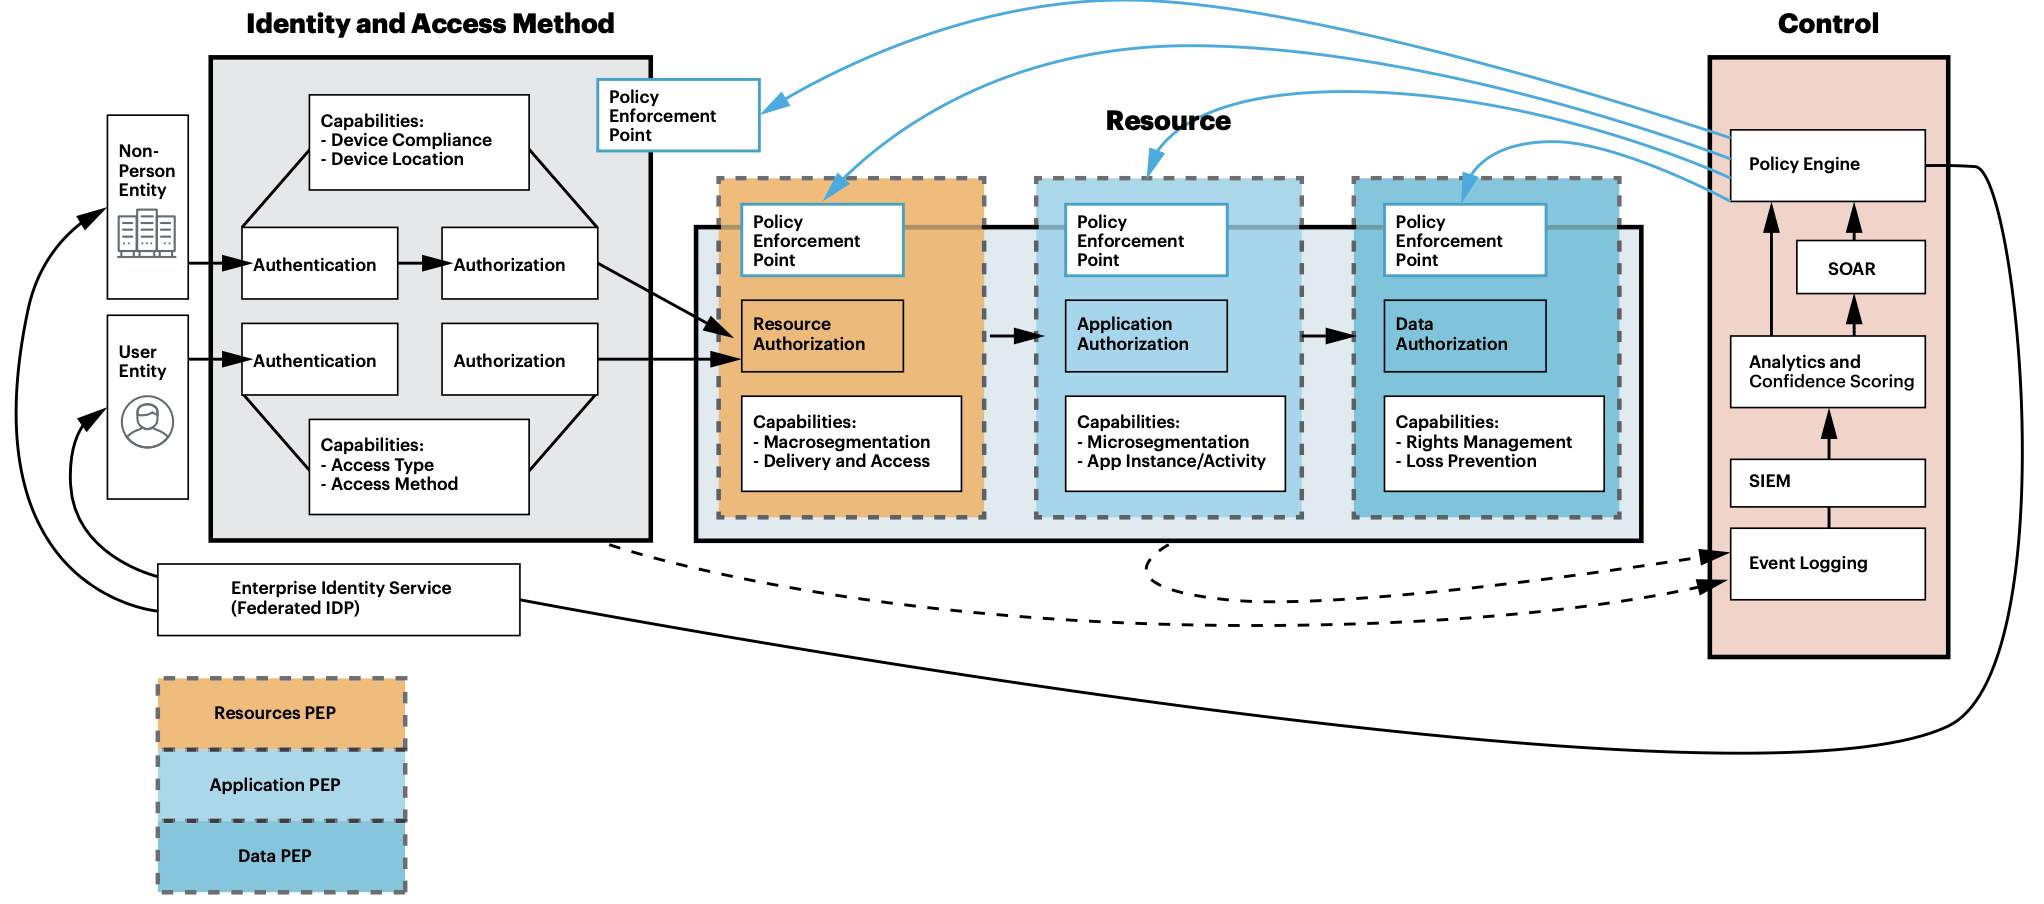
\includegraphics[width=\textwidth]{Netskope-PEP.png}
  \caption[Netskope Policy Enforcement Points (PEPs)]{Policy Enforcement Points (PEPs) in Netskope's Zero Trust Security Service Edge (SSE) platform~\autocite{Netskope2024}}
  \label{fig:Netskope-PEP}
\end{figure}


Netskope's platform integreert deze technologieën in een uitgebreid security framework dat onder andere bestaat uit:

\begin{itemize}
  \item Device en user authenticatie via een client certificaat infrastructuur
  \item Data Loss Prevention (DLP) met meer dan 3000 data identifiers en 1400 bestandstypes
  \item Software Defined WAN (SD-WAN) voor het samenvoegen van netwerken op site's met de cloud.
  \item Real-time threat protection met meer dan 40 threat intelligence feeds
\end{itemize}

Figuur~\ref{fig:Netskope-user-and-device} beschrijft het uitgebreide authenticatie- en validatieproces voor gebruikers en apparaten binnen de Netskope Zero Trust implementatie. 

\vspace{2ex}

De workflow begint bij een gebruiker die toegang vraagt, waarna eerst de apparaatconfiguratie wordt gevalideerd en de locatie wordt bepaald via on-premise detectie. Het diagram toont drie verschillende authenticatiepaden afhankelijk van het type: Domain Multi-User, Domain Single User of SAML/SSO, elk met specifieke verificatiestappen. Centrale elementen in dit proces zijn de UPN (User Principal Name) extractie voor identificatie, LDAP-gebruikersverificatie, groepsautorisatie via LDAP of SAML, en certificaatvalidatie. De Netskope Control Plane coördineert de verschillende autorisatieprocessen, past beveiligingsconfiguraties toe en zorgt voor de opzet van een versleutelde tunnel voor veilige communicatie. Rechts in het diagram worden de gebruikersattributen weergegeven die aan Netskope worden verzonden, waaronder UPN, e-mail, apparaatbeheersstatus, geïnstalleerde applicaties en diverse metadata, wat bijdraagt aan een context-bewuste beveiligingsbeoordeling in een hybride cloudscenario~\autocite{Netskope2024}.
\begin{figure}[h!]
  \centering
  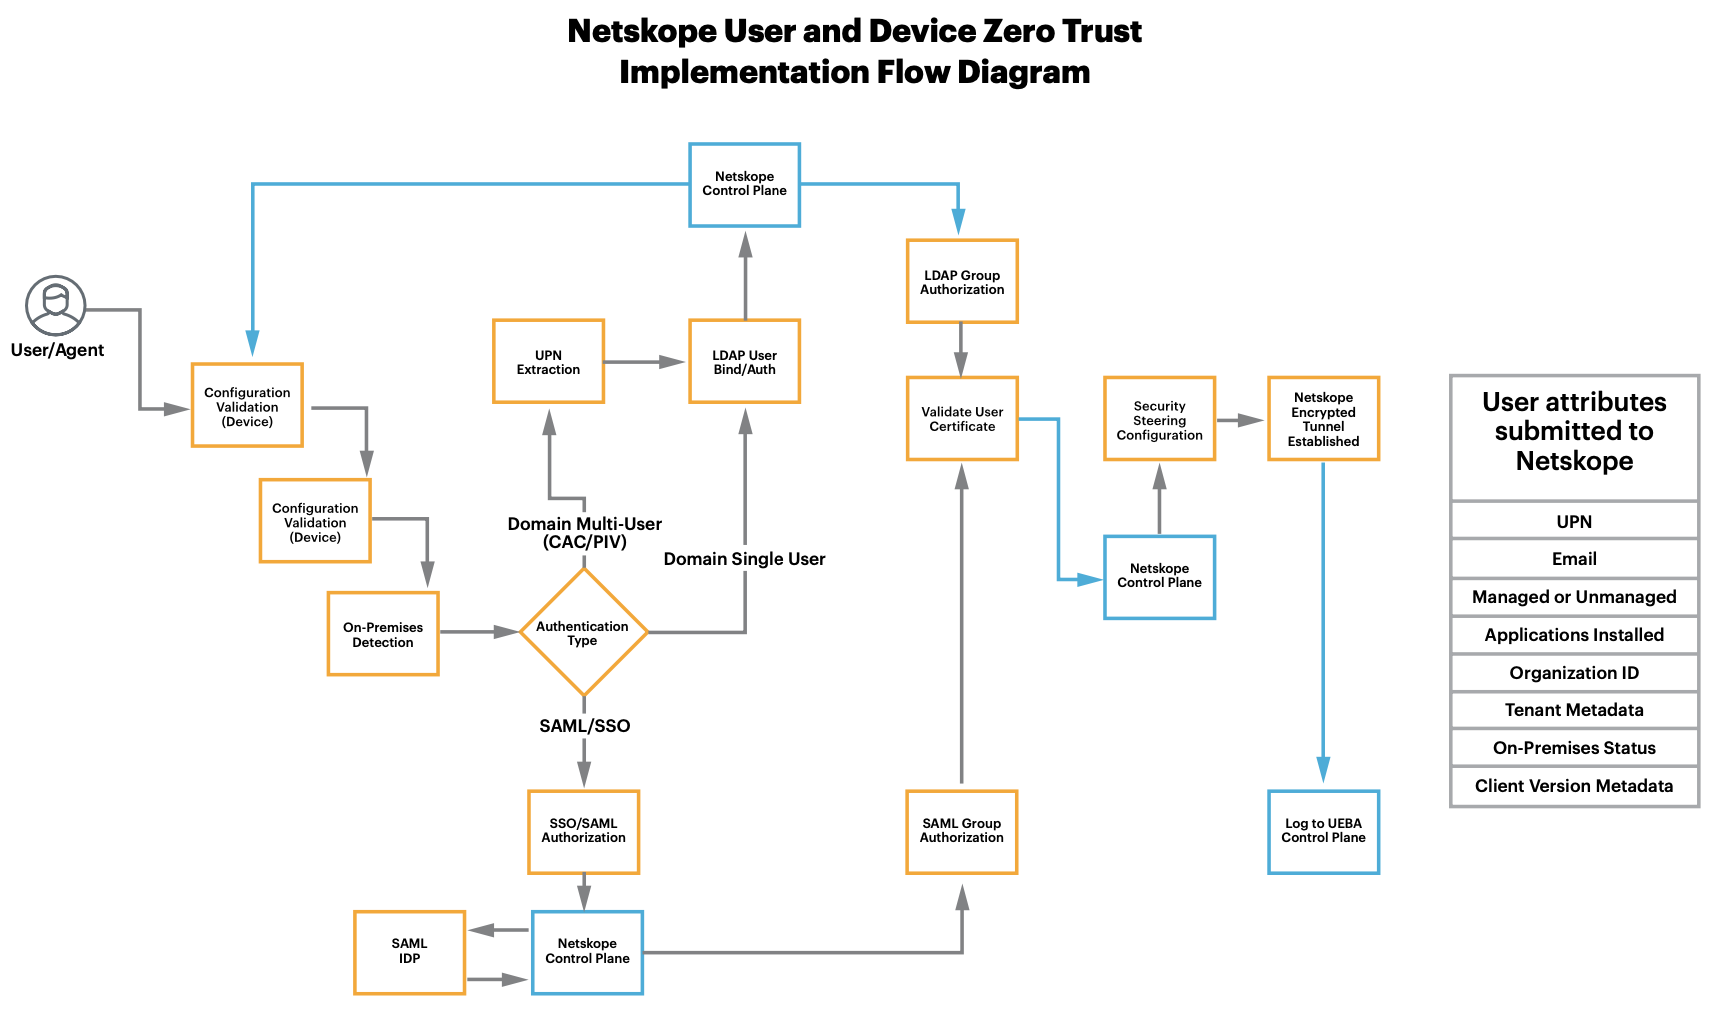
\includegraphics[width=\textwidth]{Netskope-user-and-device.png}
  \caption[Netskope Gebruiker \& Apparaat authenticatie]{Gebruiker \& Apparaat authenticatie in Netskope's Zero Trust Security Service Edge (SSE) platform~\autocite{Netskope2024}}
  \label{fig:Netskope-user-and-device}
\end{figure}

De Figuur~\ref{fig:Netskope-DLP} illustreert het Data Loss Prevention (DLP) en Digital Rights Management (DRM) implementatieproces binnen het Netskope Zero Trust raamwerk. 

\vspace{2ex}

Het proces start met een inline toegangsverzoek dat vervolgens door meerdere analyselagen gaat, beginnend met bestandsmetadata- en contentscanning, gevolgd door compliance policy evaluatie en DLP regelprofielen. Bijzonder aan deze workflow is de parallelle toepassing van zes geavanceerde analysetechnieken: Keyword Matching, Indexed Document Matching, Exact Data Matching, OCR/Fingerprinting, Image Classifiers en Text Classifiers. De Data PEP werkt als centraal beslissingspunt dat op basis van Booleaanse logica bepaalt welke actie moet worden ondernomen. De mogelijke uitkomsten omvatten directe toegang (Allow), toegangsweigering (Block), remediëring met extra beveiligingsmaatregelen zoals multi-factor authenticatie of encryptie, of beperkte toegang met uitzonderingen. 

\vspace{2ex}

Dit gehele proces vormt een diepgaande beveiligingslaag die specifiek gericht is op databescherming en preventie van datalekken binnen het SASE-architectuurraamwerk~\autocite{Netskope2024}.
\begin{figure}[h!]
  \centering
  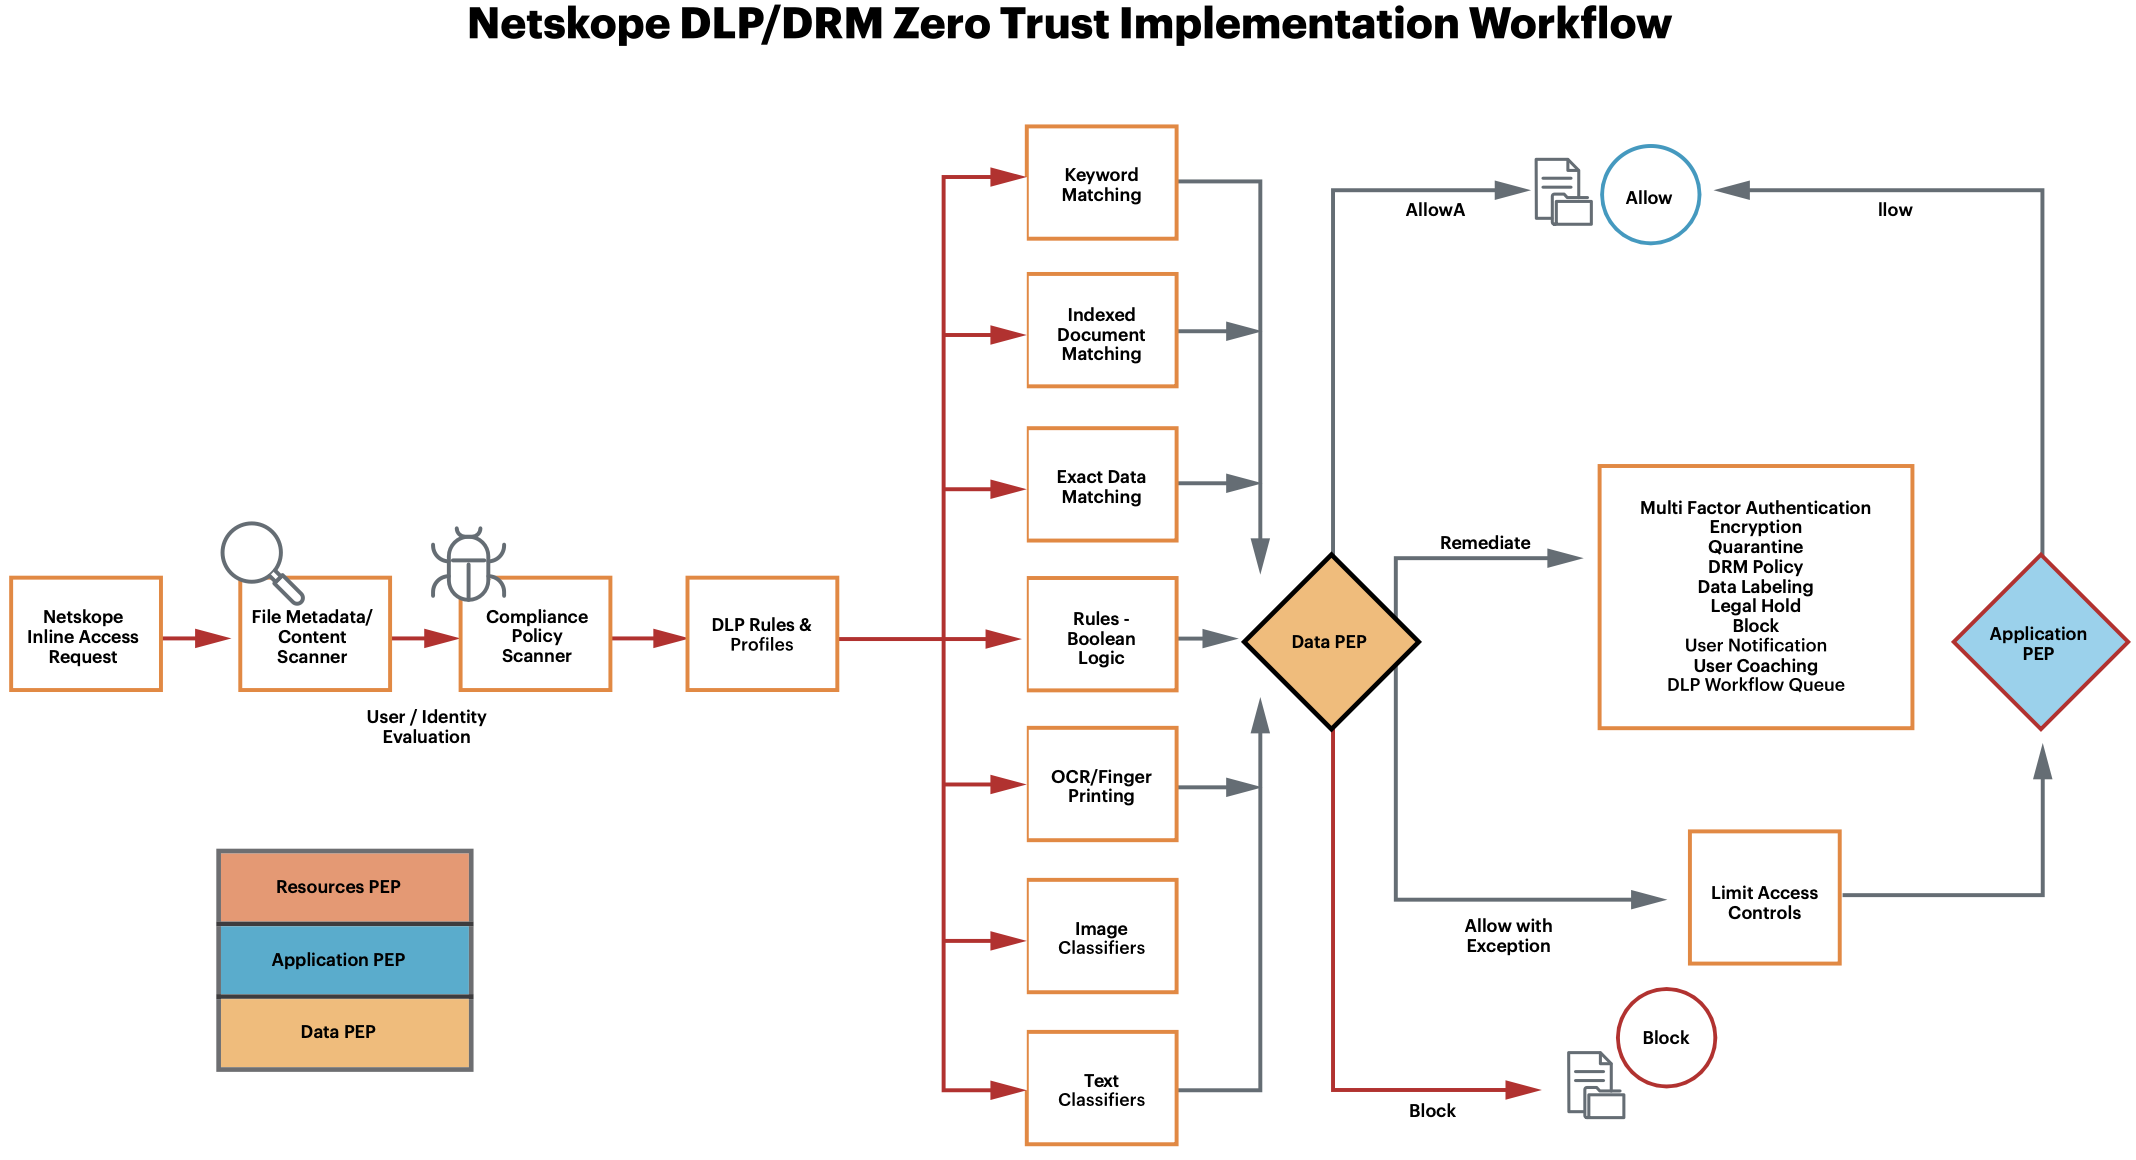
\includegraphics[width=\textwidth]{Netskope-DLP.png}
  \caption[Netskope Data Loss Prevention (DLP)]{Data Loss Prevention (DLP) in Netskope's Zero Trust Security Service Edge (SSE) platform~\autocite{Netskope2024}}
  \label{fig:Netskope-DLP}
\end{figure}

Figuur~\ref{fig:Netskope-SD-WAN} toont een gedetailleerd stroomdiagram voor de implementatie van Zero Trust principes binnen een Software-Defined Wide Area Network (SD-WAN) omgeving met Netskope. 

\vspace{2ex}

De workflow begint bij een entiteit die toegang zoekt tot een applicatie en doorloopt vervolgens verschillende beveiligingslagen. 

\vspace{2ex}

Eerst vindt device- en gebruikersverificatie plaats via het Netskope Control Plane, gevolgd door authenticatie en autorisatie. Na succesvolle authenticatie wordt de verbinding via een SD-WAN Endpoint geleid en een Port 443 Tunnel opgezet. Het cruciale beslissingspunt is de Resource PEP (Policy Enforcement Point) die evalueert of toegang moet worden verleend op basis van vooraf gedefinieerde beveiligingsregels. Bij goedkeuring wordt de verbinding via de Netskope Stitcher doorgestuurd naar de SD-WAN Publisher die de verbinding beschikbaar maakt op het oorspronkelijke protocol/poort voor de applicatie. Bij afwijzing wordt de toegang geblokkeerd, de gebruiker genotificeerd, activiteiten gelogd en risicobeoordelingen bijgewerkt~\autocite{Netskope2024}.
\begin{figure}[h!]
  \centering
  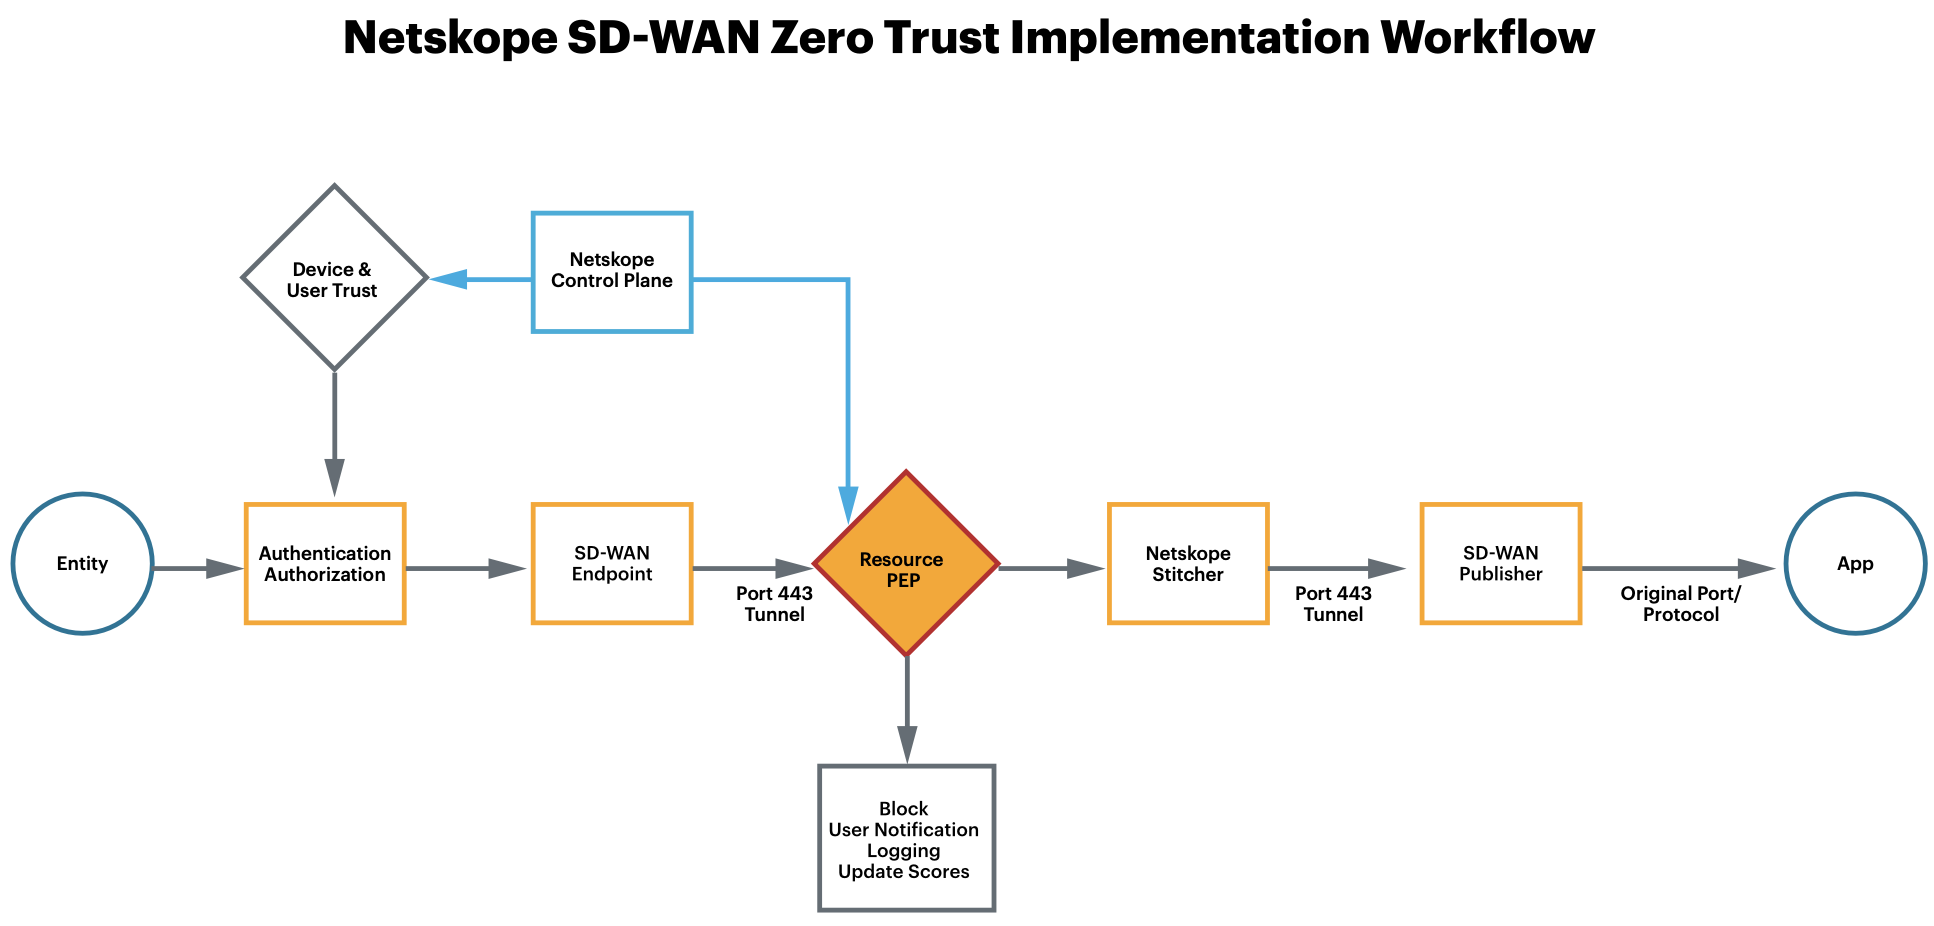
\includegraphics[width=\textwidth]{Netskope-SD-WAN.png}
  \caption[Netskope Software Defined WAN (SD-WAN)]{Software Defined WAN (SD-WAN) in Netskope's Zero Trust Security Service Edge (SSE) platform~\autocite{Netskope2024}}
  \label{fig:Netskope-SD-WAN}
\end{figure}

\vspace{2ex}

Uit onderzoek van MIT Lincoln Laboratory~\autocite{MIT2022} blijkt dat Zero Trust-architecturen bijzonder effectief zijn tegen insiderdreigingen, zoals misbruik van gecompromitteerde credentials of onbevoegde toegang door eigen medewerkers. 
Dit risico is relevant voor het onderzochte bedrijf, waar ontwikkelaars en externe partners toegang hebben tot gevoelige klantdata. 

\vspace{2ex}

MIT benadrukt dat een succesvolle Zero Trust-implementatie niet alleen technologische verandering vereist (zoals granular access control), maar ook organisatorische aanpassingen, zoals het trainen van medewerkers en het opstellen van een duidelijk beleid voor toegangsverificatie. 
Dit sluit aan bij Netskope’s focus op User \& Device workflows en gedragsanalyse, waarbij continue verificatie van gebruikers en apparaten centraal staat. 
Tegelijkertijd waarschuwt MIT voor de complexiteit van hybride implementaties, waarbij on-premises systemen en clouddiensten geïntegreerd moeten worden—een uitdaging die het bedrijf direct ondervindt en waar Netskope’s SSE-platform een antwoord op biedt.

\vspace{2ex}

Netskope biedt hiervoor een gestructureerde aanpak met specifieke operationele workflows:
\begin{itemize}
  \item \textbf{User/Device workflow}: voor initiële authenticatie en continue validatie
  \item \textbf{Network/Resource workflow}: voor toegangscontrole en segmentatie
  \item \textbf{Data Protection workflow}: voor databescherming en compliance
\end{itemize}

\vspace{2ex}

Het onderzoek van Mutemwa et al~\autocite{ACM2021} levert een belangrijke bijdrage aan ons begrip van de veranderende aard van cybersecurity in een post-pandemische wereld. Hun studie bevestigt dat traditionele perimeterbescherming fundamenteel is uitgedaagd door de verschuiving naar gedistribueerde werkomgevingen.
De auteurs besluiten dat organisaties moeten evolueren van een perimeter-gebaseerd beveiligingsmodel naar een meer complete benadering die rekening houdt met de realiteit van een uitgebreide, doorlatende bedrijfsgrens. Dit vereist een heroverweging van beveiligingsarchitecturen, met grotere nadruk op identiteitsbeheer, endpoint-beveiliging en gebruikerseducatie.

\vspace{2ex}

Deze studie onderstreept de noodzaak voor organisaties om hun cybersecurity-strategieën aan te passen aan een wereld waarin de traditionele grenzen tussen “binnen” en “buiten” het bedrijfsnetwerk steeds vager worden, een conclusie die aansluit bij de bredere verschuiving in de richting van zero-trust beveiligingsmodellen in de cybersecurity-gemeenschap.